\documentclass[10pt,first,firstsupp,handout]{THG_slides}

% Options for beamer:
%
% 9,10,11,12,13,14,17pt  Fontsizes
% 
% compress: navigation bar becomes smaller
% t       : place contents of frames on top (alternative: b,c)
% handout : handoutversion
% notes   : show notes
% notes=onlyslideswithnotes
%

\setbeamertemplate{note page}{\ \\[.3cm]
\textbf{\color{blue}Notes:}\\%[0.1cm]
{\footnotesize %\tiny
\insertnote}}

% URLs
\usepackage{url}

%% Spacing adjustments
\usepackage{textcomp} % Must be loaded to prevent conflict microtype/siunitx
\usepackage{microtype}

% Nicer tabs
\usepackage{booktabs}

%% TikZ
\usepackage{tikz}
\usepackage{gnuplot-lua-tikz}
\usetikzlibrary{tikzmark, calc, patterns, shapes, positioning,arrows,
  decorations.pathmorphing, decorations.pathreplacing, decorations.text,
  math, trees, shadows}

% Tikz macros
\tikzset{%
  highlight/.style={rectangle,rounded corners,draw,thick}
}
\newcommand{\tablearrowright}[4]{%
  \tikz[overlay,remember picture]{
  \draw ($(pic cs:#1) + (5pt,4pt)$) edge[bend right=45,-stealth]
        ($(pic cs:#2) + (5pt,4pt)$)
        node [highlight,right,xshift=5pt,yshift=7pt,#4] {#3};}
}
\newcommand{\tablearrowleft}[4]{%
  \tikz[overlay,remember picture]{
  \draw ($(pic cs:#1) + (5pt,2pt)$) edge[bend left=45,-stealth]
        ($(pic cs:#2) + (5pt,2pt)$)
        node [highlight,right,xshift=5pt,yshift=-7pt,#4] {#3};}
}
\newcommand*{\yellowemph}[1]{%
  \tikz[baseline=(X.base)] \node[rectangle, fill=yellow, rounded corners, inner sep=0.3mm] (X) {#1};%
}
\newcommand{\smiley}{%
  \tikz[baseline=-0.75ex,black]{
    \draw circle (2mm);
    \node[fill,circle,inner sep=0.5pt] (left eye) at (135:0.8mm) {};
    \node[fill,circle,inner sep=0.5pt] (right eye) at (45:0.8mm) {};
    \draw (-145:0.9mm) arc (-120:-60:1.5mm);
  }
}

% Additional colors
\usepackage{xcolor}
\colorlet{paperblue}{-red!75!green!50}

% SI units
\usepackage{siunitx}
\sisetup{per-mode = symbol, binary-units = true}
\providecommand{\gbps}[1]{\SI{#1}{\giga\byte\per\second}}
\providecommand{\mbps}[1]{\SI{#1}{\mega\byte\per\second}}
\providecommand{\gb}[1]{\SI{#1}{\giga\byte}}
\providecommand{\mb}[1]{\SI{#1}{\mega\byte}}
\providecommand{\kb}[1]{\SI{#1}{\kilo\byte}}

%\usepackage[format=hang,labelfont=bf,labelsep=space,font=small]{caption}

% Code snippets
\usepackage{listings}
\def\lstsetc{\lstset{language=C,
%  numbers=left,
%  xleftmargin=2.2em,
  xleftmargin=1.8em,
  framexleftmargin=0.2em,
  numberstyle=\tiny\color{gray},
  stepnumber=1,
  showspaces=false, 
  showstringspaces=false,
  breaklines=true,
  basicstyle=\footnotesize\ttfamily,
  stringstyle=\itshape,
  commentstyle=\itshape\bfseries,
  frame=leftline,
  morekeywords={main, size_t, malloc, free, write, H5Screate_simple},
  morekeywords={[2]H5S_UNLIMITED},
  keywordstyle={[2]\color{gray}\bfseries}
  }
}

% Shows only the navigational symbol for navigating frames.
\setbeamertemplate{navigation symbols}[only frame symbol] 

\setlayoutscale{0.5}
\setparametertextfont{\scriptsize}
\setlabelfont{\scriptsize}

\AtBeginSection[]
{
  \frame{
    \frametitle{Outline}
    \tableofcontents[currentsection]
  }
}

\begin{document}

\title{Extending HDF5 Datasets: Enhancements to the Chunk Indexing Methods}
\author{Vailin Choi, Jerome Soumagne, Quincey Koziol}
\institute{The HDF Group}

\begin{frame}
\maketitle
\end{frame}


%%%%%%%%%%%%%%%%%%%%%%%%%%%%%%%%%%%%%%%%%%%%%%%%%%%%%%%%%%%%%%%%%%%%%%%%%%%%%%%%
% Introduction
%%%%%%%%%%%%%%%%%%%%%%%%%%%%%%%%%%%%%%%%%%%%%%%%%%%%%%%%%%%%%%%%%%%%%%%%%%%%%%%%
%\section{Introduction}

\frame{
  \frametitle{Introduction}
  \begin{itemize}
    \item HDF5 Chunking is used for
  \begin{itemize}
    \item Compression
    \item I/O optimization
    \item \textbf{Extending datasets} efficiently
  \end{itemize}
  \end{itemize}

  \begin{itemize}
    \item Chunks must be indexed so that data can be retrieved efficiently
    \item Map of coordinates associated to chunk elements
  \end{itemize}
}

\frame{
  \frametitle{Chunk Indexing}
  \begin{itemize}
    \item Currently uses B-tree structure
    \item Insertion/lookup in $O(\log_b{n})$, where $n$ is the number of nodes and $b$ the order of the tree
    \item Record in B-tree stores
    \begin{itemize}
      \item Coordinates of the chunk in the dataset's dataspace.
      \item The size of the chunk, in bytes.
      \item The address of the chunk in the file.
      \item Additional metadata.
    \end{itemize}
  \end{itemize}
}

\frame{
  \frametitle{B-Tree Issues}
  \begin{itemize}
    \item Extending dataset $=$ dataset dimension only increased at upper bound
  \end{itemize}
  \begin{center}
    \resizebox{\linewidth}{!}{
       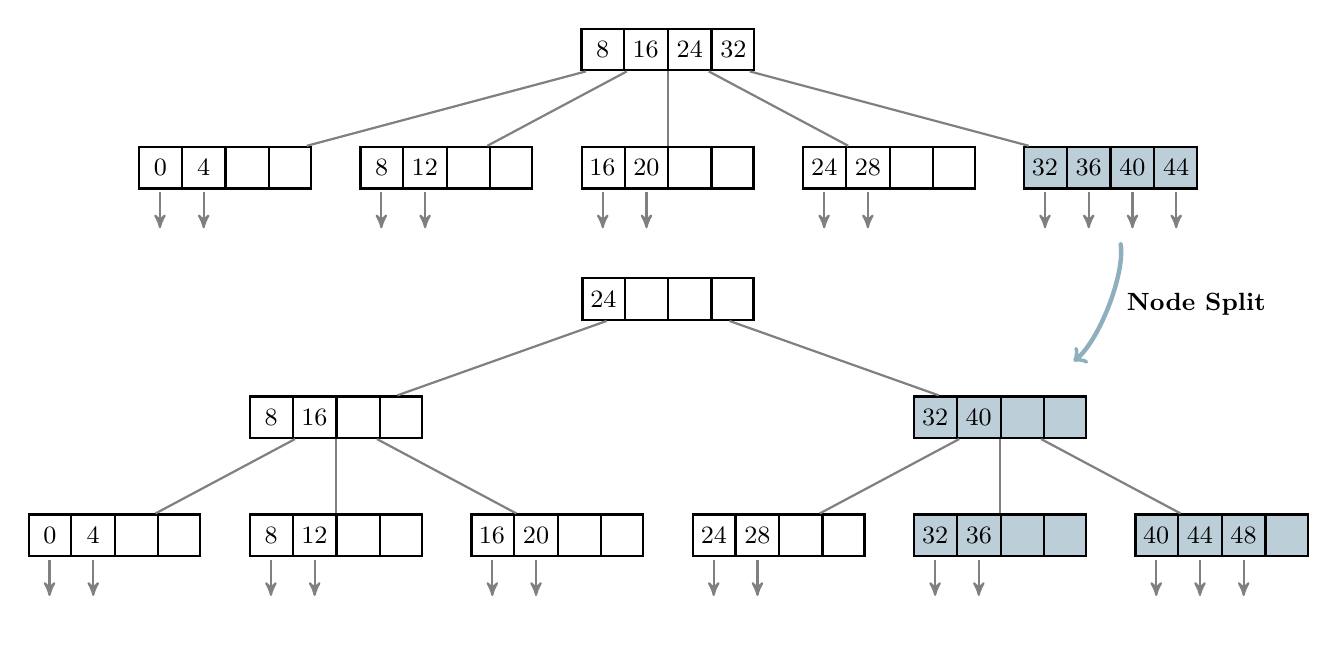
\begin{tikzpicture}
\tikzstyle{trans} = [gray,->,thick,>=stealth',shorten <=1pt,shorten >=1pt]
\tikzstyle{node_style} = [rectangle split,rectangle split horizontal,
  rectangle split parts=4,rectangle split empty part width=10.5pt,
  text width=15pt,inner sep=0,thick,draw=black,
  minimum height=15pt,text centered,anchor=center,font=\small]
\tikzstyle{edge_style} = [gray,thick,draw]
\tikzstyle{level 1}=[sibling distance=80pt]

\uncover<1->{
\begin{scope} [local bounding box=scope1,%edge from parent fork down,
  every node/.style=node_style, edge from parent/.style=edge_style]
\node {8 \nodepart{two} 16 \nodepart{three} 24 \nodepart{four} 32}
  child {node (l1_0) {0 \nodepart{two} 4}}
  child {node (l1_1) {8 \nodepart{two} 12}}
   child {node (l1_2) {16 \nodepart{two} 20}}
   child {node (l1_3) {24 \nodepart{two} 28}}
   child {node[fill=paperblue!30] (l1_4) {32 \nodepart{two} 36 \nodepart{three} 40 \nodepart{four} 44}};
\end{scope}

\foreach \i in {0,...,4} {
\node[below=15pt of l1_\i.one south] (c\i) {};
\draw[trans] (l1_\i.one south) -- (c\i);
\node[below=15pt of l1_\i.two south] (c\i_2) {};
\draw[trans] (l1_\i.two south) -- (c\i_2);
}
% Last two arrows
\node[below=15pt of l1_4.three south] (c4_3) {};
\draw[trans] (l1_4.three south) -- (c4_3);
\node[below=15pt of l1_4.four south] (c4_4) {};
\draw[trans] (l1_4.four south) -- (c4_4);
}

\uncover<3->{
\begin{scope}[shift={($(scope1.south)+(0,-40pt)$)},%edge from parent fork down,
  every node/.style=node_style, edge from parent/.style=edge_style]
\tikzstyle{level 1}=[sibling distance=240pt]
\tikzstyle{level 2}=[sibling distance=80pt]
\node {24}
  child {node {8 \nodepart{two} 16}
    child {node (l2_0) {0 \nodepart{two} 4}}
    child {node (l2_1) {8 \nodepart{two} 12}}
    child {node (l2_2) {16 \nodepart{two} 20}}
  }
  child {node[fill=paperblue!30] (l2_split) {32 \nodepart{two} 40}
    child {node (l2_3) {24 \nodepart{two} 28}}
    child {node[fill=paperblue!30] (l2_4) {32 \nodepart{two} 36}}
    child {node[fill=paperblue!30] (l2_5) {40 \nodepart{two} 44 \nodepart{three} 48}}
  };
\end{scope}

\foreach \i in {0,...,5} {
\node[below=15pt of l2_\i.one south] (c\i) {};
\draw[trans] (l2_\i.one south) -- (c\i);
\node[below=15pt of l2_\i.two south] (c\i_2) {};
\draw[trans] (l2_\i.two south) -- (c\i_2);
}
% Last arrow
\node[below=15pt of l2_5.three south] (c5_3) {};
\draw[trans] (l2_5.three south) -- (c5_3);
}

\uncover<2->{
\draw[overlay,remember picture,ultra thick,line cap=round,->,
  draw=paperblue!50,shorten <=20pt,shorten >=20pt] (l1_4) to [bend left=30]
  node[right=5pt, font=\small\bfseries] {Node Split} 
  (l2_split);
}
\end{tikzpicture}


    }
  \end{center}
}

\frame{
  \frametitle{B-Tree Issues}
  \begin{itemize}
    \item B-tree v2 fixes re-balancing issue
    \item More optimizations \textit{tweaks} but same complexity
    \item B-tree not ideal for dataset extended in single dimension
    \begin{itemize}
      \item Use extensible array instead
    \end{itemize}
  \end{itemize}
}


\frame{
  \frametitle{Extensible Array}
  \begin{itemize}
    \item Insertion/removal/lookup in $O(1)$
  \end{itemize}
  \begin{center}
    \resizebox{\linewidth}{!}{
       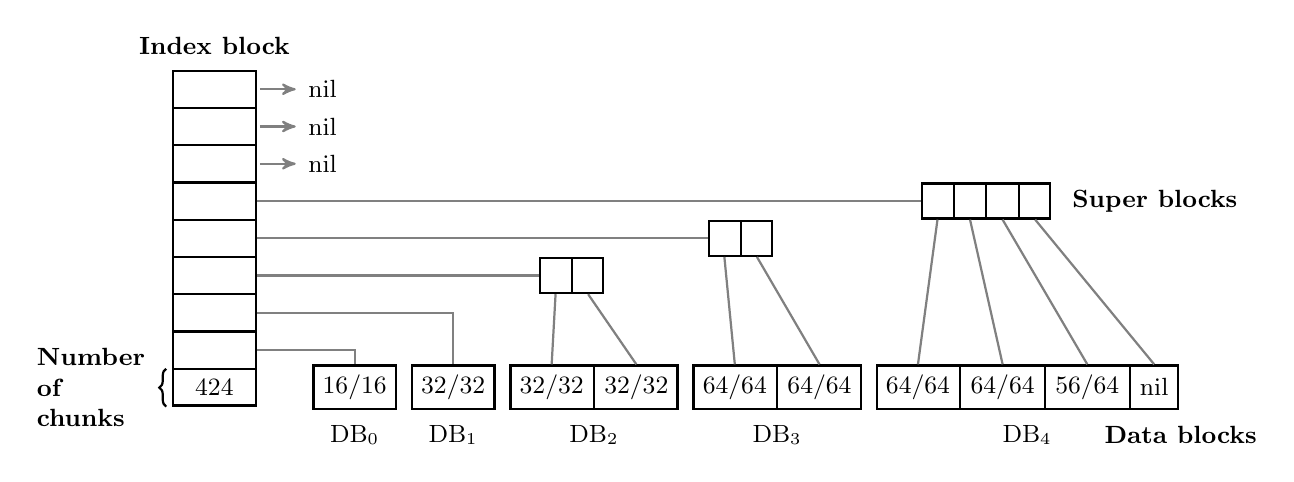
\begin{tikzpicture}
\tikzstyle{sblock} = [rectangle split,rectangle split horizontal,
  rectangle split empty part height=6pt,thick,draw=black,
  minimum width=30pt,text centered,font=\small,
  anchor=center]
\tikzstyle{iblock} = [rectangle split,rectangle split parts=9,
  rectangle split empty part height=6pt,thick,draw=black,
  minimum width=30pt,text centered,font=\small,
  anchor=center]
\tikzstyle{link} = [gray,thick,draw]
\tikzstyle{trans} = [gray,->,thick,>=stealth',shorten <=1pt,shorten >=1pt]
\tikzstyle{annotation} = [font=\small]

\node[iblock] (index) {~\nodepart{two}~\nodepart{three}~\nodepart{four}~\nodepart{five}~\nodepart{six}~\nodepart{seven}~\nodepart{eight}~\nodepart{nine}424};
\node[sblock,rectangle split parts=1,right=20pt of index.nine east] (sblock0) {16/16};
\node[sblock,rectangle split parts=1,right=5pt of sblock0] (sblock1) {32/32};
\node[sblock,rectangle split parts=2,right=5pt of sblock1] (sblock2) {32/32 \nodepart{two} 32/32};
\node[sblock,rectangle split parts=2,right=5pt of sblock2] (sblock3) {64/64 \nodepart{two} 64/64};
\node[sblock,rectangle split parts=4,right=5pt of sblock3] (sblock4) {64/64 \nodepart{two} 64/64 \nodepart{three} 56/64 \nodepart{four} nil};
\node[sblock,rectangle split parts=2,right=102pt of index.six east] (sblock2b) {};
\node[sblock,rectangle split parts=2,right=163pt of index.five east] (sblock3b) {};
\node[sblock,rectangle split parts=4,right=240pt of index.four east] (sblock4b) {};

\draw[link] (index.eight east) -| (sblock0);
\draw[link] (index.seven east) -| (sblock1);
\draw[link] (index.six east) -- (sblock2b);
\draw[link] (index.five east) -- (sblock3b);
\draw[link] (index.four east) -- (sblock4b);

\draw[link] (sblock2b.one south) -- (sblock2.one north);
\draw[link] (sblock2b.two south) -- (sblock2.two north);

\draw[link] (sblock3b.one south) -- (sblock3.one north);
\draw[link] (sblock3b.two south) -- (sblock3.two north);

\draw[link] (sblock4b.one south) -- (sblock4.one north);
\draw[link] (sblock4b.two south) -- (sblock4.two north);
\draw[link] (sblock4b.three south) -- (sblock4.three north);
\draw[link] (sblock4b.four south) -- (sblock4.four north);

\node[annotation,right=15pt of index.one east] (nil0) {nil};
\draw[trans] (index.one east) -- (nil0);
\node[annotation,right=15pt of index.two east] (nil1) {nil};
\draw[trans] (index.two east) -- (nil1);
\node[annotation,right=15pt of index.three east] (nil2) {nil};
\draw[trans] (index.three east) -- (nil2);

\uncover<3->{
\draw[decorate,decoration={brace,mirror,raise=2pt}, thick] (index.eight split west) to node [annotation,text width=40pt,left=5pt,font=\small\bfseries] {Number of chunks} (index.south west);
}
\node[annotation,below=2pt of sblock0] {DB$_0$};
\node[annotation,below=2pt of sblock1] {DB$_1$};
\node[annotation,below=2pt of sblock2] {DB$_2$};
\node[annotation,below=2pt of sblock3] {DB$_3$};
\node[annotation,below=2pt of sblock4] (sblock4_annotation) {DB$_4$};
\uncover<2->{
\node[annotation,above=2pt of index,font=\small\bfseries] {Index block};
}
\uncover<5->{
\node[annotation,right=12pt of sblock4_annotation,font=\small\bfseries] {Data blocks};
}
\uncover<4->{
\node[annotation,right=4pt of sblock4b,font=\small\bfseries] {Super blocks};
}

% To help center
%\node[above=100pt of sblock2.one split] (help2) {};
%\draw (help2) -- (sblock2.one split);
%\node[above=100pt of sblock3.one split] (help3) {};
%\draw (help3) -- (sblock3.one split);
%\node[above=100pt of sblock4.two split] (help4) {};
%\draw (help4) -- (sblock4.two split);
\end{tikzpicture}


    }
  \end{center}
}

\frame{
  \frametitle{Hash Table}
  \begin{itemize}
    \item Chunk present in cache are retrieved from cache hash table
    \item Each entry hashed based on the chunk index (varies according to dataset
    dimension size)
    \item Extending dataset means
    \begin{itemize}
      \item Recalculation of every hash value \yellowemph{EVERY TIME}
    \end{itemize}
  \end{itemize}
}

\frame{
  \frametitle{Hashing Chunks Coordinates}
  \begin{center}
    \resizebox{\linewidth}{!}{
       \tikzstyle{trans} = [>=stealth, thick, text centered, font=\small]
\tikzstyle{computBox} = [draw=black, thick, inner sep=4pt, inner ysep=4pt,
  rectangle, rounded corners]

\newcommand{\drawcuboid}[5]{% width, height, depth, scale, color
\begin{scope}[scale=#4]
\coordinate (O) at (0,0,0);
\coordinate (A) at (0,#2,0);
\coordinate (B) at (0,#2,#3);
\coordinate (C) at (0,0,#3);
\coordinate (D) at (#1,0,0);
\coordinate (E) at (#1,#2,0);
\coordinate (F) at (#1,#2,#3);
\coordinate (G) at (#1,0,#3);

\draw[fill=#5] (O) -- (C) -- (G) -- (D) -- cycle;% Bottom Face
\draw[fill=#5] (O) -- (A) -- (E) -- (D) -- cycle;% Back Face
\draw[fill=#5] (O) -- (A) -- (B) -- (C) -- cycle;% Left Face
\draw[fill=#5] (D) -- (E) -- (F) -- (G) -- cycle;% Right Face
\draw[fill=#5] (C) -- (B) -- (F) -- (G) -- cycle;% Front Face
\draw[fill=#5] (A) -- (B) -- (F) -- (E) -- cycle;% Top Face

\draw[dashed] (O) -- (D);
\draw[dashed] (O) -- (C);
\draw[dashed] (O) -- (A);

\coordinate[left=6pt of A] (A1);
\coordinate[left=6pt of B] (B1);
\coordinate[left=6pt of C] (C1);
\coordinate[below=4pt of C] (C2);
\coordinate[below=4pt of G] (G1);
\draw[<->,trans] (C2) -- node [below] {#1} (G1);
\draw[<->,trans] (C1) -- node [left] {#2} (B1);
\draw[<->,trans] (A1) -- node [above left] {#3} (B1);

\end{scope}
}

%\DeclarePairedDelimiter\ceil{\lceil}{\rceil}

\begin{tikzpicture}

\node (cubes) {
\begin{minipage}{0.32\textwidth}
\begin{tikzpicture}
% Origin axes
\draw[->,draw=paperblue,thick] (0,0,0) -- (3.2,0,0);
\draw[->,draw=paperblue,thick] (0,0,0) -- (0,3.8,0);
\draw[->,draw=paperblue,thick] (0,0,0) -- (0,0,4);
\node[font=\itshape] at (3.4,0,0) {x};
\node[font=\itshape] at (0,4,0) {y};
\node[font=\itshape] at (0,0,4.2) {z};

% Cubes
\drawcuboid{60}{75}{75}{0.04}{white}
\drawcuboid{10}{25}{25}{0.04}{paperblue!20}
\end{tikzpicture}
\end{minipage}
};

% Hash value computation
\node [computBox, font=\footnotesize, text width=100pt, right=50pt of cubes] (scaled) {
  \begin{minipage}{\textwidth}
  {
\textbf{Scaled coordinates:}\\
\begin{math}
   X/x = 60/10 = 6\\
   Y/y = 75/25 = 3\\
   Z/z = 75/25 = 3
\end{math}

\smallskip
\textbf{Number of bits to represent\\ coordinates:}\\
\begin{math}
   \lceil \log_2(X/x) \rceil = 3\\
   \lceil \log_2(Y/y) \rceil = 2\\
   \lceil \log_2(Z/z) \rceil = 2
\end{math}
  }
  \end{minipage}
};

\node [right=of scaled,rectangle split,rectangle split horizontal,
  rectangle split parts=2,draw, minimum height=15pt,text centered,anchor=center,font=\small] (zhash) {0 \nodepart{two} 0};
\node [right=14pt of zhash,rectangle split,rectangle split horizontal,
  rectangle split parts=2,draw, minimum height=15pt,text centered,anchor=center,font=\small] (yhash) {0 \nodepart{two} 0};
\node [right=20pt of yhash,rectangle split,rectangle split horizontal,
  rectangle split parts=3,draw, minimum height=15pt,text centered,anchor=center,font=\small] (xhash) {0 \nodepart{two} 0 \nodepart{three} 0};
\node [below=2pt of xhash] {$x$};
\node [below=2pt of yhash] {$y$};
\node [below=2pt of zhash] {$z$};

\draw[very thick, ->] (cubes) -- node[above, text width=4cm, align=center, font=\bfseries]
    {Hash-value} ($ (scaled.west) - (0.5,0) $);

\end{tikzpicture}



    }
  \end{center}
}

\frame{
  \frametitle{Chunk Indexing Performance}
\begin{columns}[c] % the "c" option specifies center vertical alignment
\column{.5\textwidth}
\begin{itemize}
\item Before
\end{itemize}
\resizebox{\linewidth}{!}{
\uncover<2->{
\begin{tabular}{lrr} \toprule
Indexing Method &
Time (\si{\second}) \\
\midrule
\textit{Along the X-direction} \\
EA & $149.82$\tikzmark{t1x1} \\
BT1 & $156.15$\tikzmark{t1x2} \\
BT2 & $166.56$\tikzmark{t1x3} \\
\midrule
\textit{Along the Y-direction} \\
EA & $150.08$\tikzmark{t1y1} \\
BT1 & $163.82$\tikzmark{t1y2} \\
BT2 & $167.91$\tikzmark{t1y3} \\
\midrule
\textit{Along the XY-direction} \\
EA & $-$ \\
BT1 & $104.08$\tikzmark{t1xy1} \\
BT2 & $114.39$\tikzmark{t1xy2} \\
\bottomrule
\end{tabular}
}
\uncover<3->{
\tablearrowright{t1x2}{t1x1}{$\simeq -4\%$}{}
\tablearrowleft{t1x2}{t1x3}{$\simeq +7\%$}{}
\tablearrowright{t1y2}{t1y1}{$\simeq -8\%$}{}
\tablearrowleft{t1y2}{t1y3}{$\simeq +2\%$}{}
\tablearrowleft{t1xy1}{t1xy2}{$\simeq +10\%$}{}
}
}
\column{.5\textwidth}
\uncover<4->{
\begin{itemize}
\item After
\end{itemize}
}
\resizebox{\linewidth}{!}{
\uncover<5->{
\begin{tabular}{lr} \toprule
Indexing Method &
Time (\si{\second}) \\
\midrule
\textit{Along the X-direction} \\
EA & $32.10$\tikzmark{x1}\\
BT1 & $36.63$\tikzmark{x2} \\
BT2 & $35.39$\tikzmark{x3} \\
\midrule
\textit{Along the Y-direction} \\
EA & $32.2$\tikzmark{y1} \\
BT1 & $39.01$\tikzmark{y2} \\
BT2 & $34.90$\tikzmark{y3} \\
\midrule
\textit{Along the XY-direction} \\
EA & $-$ \\
BT1 & $36.11$\tikzmark{xy1} \\
BT2 & $35.29$\tikzmark{xy2} \\
\bottomrule
\end{tabular}
}
\uncover<6->{
\tablearrowright{x2}{x1}{$\simeq -12.4\%$}{}
\tablearrowleft{x2}{x3}{$\simeq -3.4\%$}{fill=paperblue!30}
\tablearrowright{y2}{y1}{$\simeq -17.5\%$}{}
\tablearrowleft{y2}{y3}{$\simeq -10.5\%$}{fill=paperblue!30}
\tablearrowleft{xy1}{xy2}{$\simeq -2.3\%$}{fill=paperblue!30}
}
}
\end{columns}
}

\frame{
  \frametitle{Chunk Indexing Performance}
  \begin{center}
    \resizebox{\linewidth}{!}{
       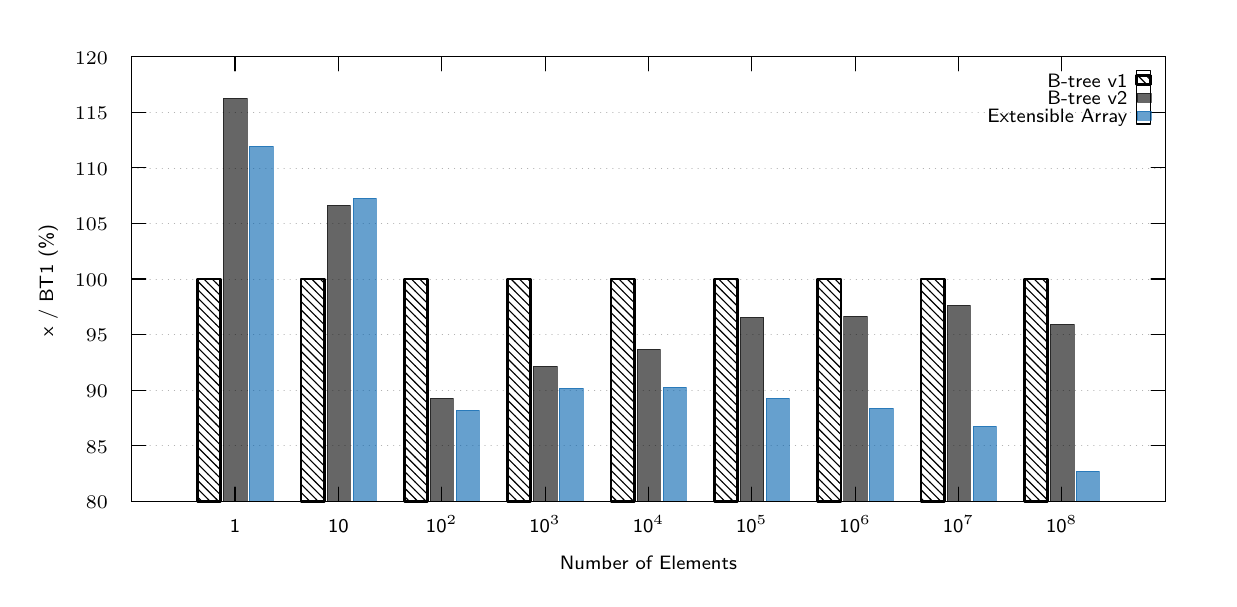
\begin{tikzpicture}[gnuplot]
%% generated with GNUPLOT 5.0p0 (Lua 5.3; terminal rev. 99, script rev. 100)
%% Tue 09 Jun 2015 04:43:46 PM CDT
\tikzset{every node/.append style={font={\sffamily\scriptsize}}}
\path (0.000,0.000) rectangle (15.000,7.000);
\gpcolor{color=gp lt color axes}
\gpsetlinetype{gp lt axes}
\gpsetdashtype{gp dt axes}
\gpsetlinewidth{0.50}
\draw[gp path] (1.320,0.985)--(14.447,0.985);
\gpcolor{color=gp lt color border}
\gpsetlinetype{gp lt border}
\gpsetdashtype{gp dt solid}
\gpsetlinewidth{1.00}
\draw[gp path] (1.320,0.985)--(1.500,0.985);
\draw[gp path] (14.447,0.985)--(14.267,0.985);
\node[gp node right,font={\sffamily\scriptsize}] at (1.136,0.985) {$80$};
\gpcolor{color=gp lt color axes}
\gpsetlinetype{gp lt axes}
\gpsetdashtype{gp dt axes}
\gpsetlinewidth{0.50}
\draw[gp path] (1.320,1.691)--(14.447,1.691);
\gpcolor{color=gp lt color border}
\gpsetlinetype{gp lt border}
\gpsetdashtype{gp dt solid}
\gpsetlinewidth{1.00}
\draw[gp path] (1.320,1.691)--(1.500,1.691);
\draw[gp path] (14.447,1.691)--(14.267,1.691);
\node[gp node right,font={\sffamily\scriptsize}] at (1.136,1.691) {$85$};
\gpcolor{color=gp lt color axes}
\gpsetlinetype{gp lt axes}
\gpsetdashtype{gp dt axes}
\gpsetlinewidth{0.50}
\draw[gp path] (1.320,2.397)--(14.447,2.397);
\gpcolor{color=gp lt color border}
\gpsetlinetype{gp lt border}
\gpsetdashtype{gp dt solid}
\gpsetlinewidth{1.00}
\draw[gp path] (1.320,2.397)--(1.500,2.397);
\draw[gp path] (14.447,2.397)--(14.267,2.397);
\node[gp node right,font={\sffamily\scriptsize}] at (1.136,2.397) {$90$};
\gpcolor{color=gp lt color axes}
\gpsetlinetype{gp lt axes}
\gpsetdashtype{gp dt axes}
\gpsetlinewidth{0.50}
\draw[gp path] (1.320,3.102)--(14.447,3.102);
\gpcolor{color=gp lt color border}
\gpsetlinetype{gp lt border}
\gpsetdashtype{gp dt solid}
\gpsetlinewidth{1.00}
\draw[gp path] (1.320,3.102)--(1.500,3.102);
\draw[gp path] (14.447,3.102)--(14.267,3.102);
\node[gp node right,font={\sffamily\scriptsize}] at (1.136,3.102) {$95$};
\gpcolor{color=gp lt color axes}
\gpsetlinetype{gp lt axes}
\gpsetdashtype{gp dt axes}
\gpsetlinewidth{0.50}
\draw[gp path] (1.320,3.808)--(14.447,3.808);
\gpcolor{color=gp lt color border}
\gpsetlinetype{gp lt border}
\gpsetdashtype{gp dt solid}
\gpsetlinewidth{1.00}
\draw[gp path] (1.320,3.808)--(1.500,3.808);
\draw[gp path] (14.447,3.808)--(14.267,3.808);
\node[gp node right,font={\sffamily\scriptsize}] at (1.136,3.808) {$100$};
\gpcolor{color=gp lt color axes}
\gpsetlinetype{gp lt axes}
\gpsetdashtype{gp dt axes}
\gpsetlinewidth{0.50}
\draw[gp path] (1.320,4.514)--(14.447,4.514);
\gpcolor{color=gp lt color border}
\gpsetlinetype{gp lt border}
\gpsetdashtype{gp dt solid}
\gpsetlinewidth{1.00}
\draw[gp path] (1.320,4.514)--(1.500,4.514);
\draw[gp path] (14.447,4.514)--(14.267,4.514);
\node[gp node right,font={\sffamily\scriptsize}] at (1.136,4.514) {$105$};
\gpcolor{color=gp lt color axes}
\gpsetlinetype{gp lt axes}
\gpsetdashtype{gp dt axes}
\gpsetlinewidth{0.50}
\draw[gp path] (1.320,5.220)--(14.447,5.220);
\gpcolor{color=gp lt color border}
\gpsetlinetype{gp lt border}
\gpsetdashtype{gp dt solid}
\gpsetlinewidth{1.00}
\draw[gp path] (1.320,5.220)--(1.500,5.220);
\draw[gp path] (14.447,5.220)--(14.267,5.220);
\node[gp node right,font={\sffamily\scriptsize}] at (1.136,5.220) {$110$};
\gpcolor{color=gp lt color axes}
\gpsetlinetype{gp lt axes}
\gpsetdashtype{gp dt axes}
\gpsetlinewidth{0.50}
\draw[gp path] (1.320,5.925)--(14.083,5.925);
\draw[gp path] (14.263,5.925)--(14.447,5.925);
\gpcolor{color=gp lt color border}
\gpsetlinetype{gp lt border}
\gpsetdashtype{gp dt solid}
\gpsetlinewidth{1.00}
\draw[gp path] (1.320,5.925)--(1.500,5.925);
\draw[gp path] (14.447,5.925)--(14.267,5.925);
\node[gp node right,font={\sffamily\scriptsize}] at (1.136,5.925) {$115$};
\gpcolor{color=gp lt color axes}
\gpsetlinetype{gp lt axes}
\gpsetdashtype{gp dt axes}
\gpsetlinewidth{0.50}
\draw[gp path] (1.320,6.631)--(14.447,6.631);
\gpcolor{color=gp lt color border}
\gpsetlinetype{gp lt border}
\gpsetdashtype{gp dt solid}
\gpsetlinewidth{1.00}
\draw[gp path] (1.320,6.631)--(1.500,6.631);
\draw[gp path] (14.447,6.631)--(14.267,6.631);
\node[gp node right,font={\sffamily\scriptsize}] at (1.136,6.631) {$120$};
\draw[gp path] (2.633,0.985)--(2.633,1.165);
\draw[gp path] (2.633,6.631)--(2.633,6.451);
\node[gp node center,font={\sffamily\scriptsize}] at (2.633,0.677) {1};
\draw[gp path] (3.945,0.985)--(3.945,1.165);
\draw[gp path] (3.945,6.631)--(3.945,6.451);
\node[gp node center,font={\sffamily\scriptsize}] at (3.945,0.677) {10};
\draw[gp path] (5.258,0.985)--(5.258,1.165);
\draw[gp path] (5.258,6.631)--(5.258,6.451);
\node[gp node center,font={\sffamily\scriptsize}] at (5.258,0.677) {10$^2$};
\draw[gp path] (6.571,0.985)--(6.571,1.165);
\draw[gp path] (6.571,6.631)--(6.571,6.451);
\node[gp node center,font={\sffamily\scriptsize}] at (6.571,0.677) {10$^3$};
\draw[gp path] (7.884,0.985)--(7.884,1.165);
\draw[gp path] (7.884,6.631)--(7.884,6.451);
\node[gp node center,font={\sffamily\scriptsize}] at (7.884,0.677) {10$^4$};
\draw[gp path] (9.196,0.985)--(9.196,1.165);
\draw[gp path] (9.196,6.631)--(9.196,6.451);
\node[gp node center,font={\sffamily\scriptsize}] at (9.196,0.677) {10$^5$};
\draw[gp path] (10.509,0.985)--(10.509,1.165);
\draw[gp path] (10.509,6.631)--(10.509,6.451);
\node[gp node center,font={\sffamily\scriptsize}] at (10.509,0.677) {10$^6$};
\draw[gp path] (11.822,0.985)--(11.822,1.165);
\draw[gp path] (11.822,6.631)--(11.822,6.451);
\node[gp node center,font={\sffamily\scriptsize}] at (11.822,0.677) {10$^7$};
\draw[gp path] (13.134,0.985)--(13.134,1.165);
\draw[gp path] (13.134,6.631)--(13.134,6.451);
\node[gp node center,font={\sffamily\scriptsize}] at (13.134,0.677) {10$^8$};
\draw[gp path] (1.320,6.631)--(1.320,0.985)--(14.447,0.985)--(14.447,6.631)--cycle;
\node[gp node center,rotate=-270,font={\sffamily\scriptsize}] at (0.246,3.808) {x / BT1 (\%)};
\node[gp node center,font={\sffamily\scriptsize}] at (7.883,0.215) {Number of Elements};
\draw[gp path] (14.083,5.776)--(14.083,6.451)--(14.263,6.451)--(14.263,5.776)--cycle;
\node[gp node right,font={\sffamily\fontsize{7.0pt}{8.4pt}\selectfont}] at (14.083,6.338) {B-tree v1};
\def\gpfillpath{(14.083,6.282)--(14.263,6.282)--(14.263,6.394)--(14.083,6.394)--cycle}
\gpfill{color=gpbgfillcolor} \gpfillpath;
\gpfill{rgb color={0.000,0.000,0.000},gp pattern 2,pattern color=.} \gpfillpath;
\gpcolor{rgb color={0.000,0.000,0.000}}
\gpsetlinewidth{2.50}
\draw[gp path] (14.083,6.282)--(14.263,6.282)--(14.263,6.394)--(14.083,6.394)--cycle;
\def\gpfillpath{(2.157,0.985)--(2.453,0.985)--(2.453,3.809)--(2.157,3.809)--cycle}
\gpfill{color=gpbgfillcolor} \gpfillpath;
\gpfill{rgb color={0.000,0.000,0.000},gp pattern 2,pattern color=.} \gpfillpath;
\draw[gp path] (2.157,0.985)--(2.157,3.808)--(2.452,3.808)--(2.452,0.985)--cycle;
\def\gpfillpath{(3.470,0.985)--(3.766,0.985)--(3.766,3.809)--(3.470,3.809)--cycle}
\gpfill{color=gpbgfillcolor} \gpfillpath;
\gpfill{rgb color={0.000,0.000,0.000},gp pattern 2,pattern color=.} \gpfillpath;
\draw[gp path] (3.470,0.985)--(3.470,3.808)--(3.765,3.808)--(3.765,0.985)--cycle;
\def\gpfillpath{(4.782,0.985)--(5.079,0.985)--(5.079,3.809)--(4.782,3.809)--cycle}
\gpfill{color=gpbgfillcolor} \gpfillpath;
\gpfill{rgb color={0.000,0.000,0.000},gp pattern 2,pattern color=.} \gpfillpath;
\draw[gp path] (4.782,0.985)--(4.782,3.808)--(5.078,3.808)--(5.078,0.985)--cycle;
\def\gpfillpath{(6.095,0.985)--(6.391,0.985)--(6.391,3.809)--(6.095,3.809)--cycle}
\gpfill{color=gpbgfillcolor} \gpfillpath;
\gpfill{rgb color={0.000,0.000,0.000},gp pattern 2,pattern color=.} \gpfillpath;
\draw[gp path] (6.095,0.985)--(6.095,3.808)--(6.390,3.808)--(6.390,0.985)--cycle;
\def\gpfillpath{(7.408,0.985)--(7.704,0.985)--(7.704,3.809)--(7.408,3.809)--cycle}
\gpfill{color=gpbgfillcolor} \gpfillpath;
\gpfill{rgb color={0.000,0.000,0.000},gp pattern 2,pattern color=.} \gpfillpath;
\draw[gp path] (7.408,0.985)--(7.408,3.808)--(7.703,3.808)--(7.703,0.985)--cycle;
\def\gpfillpath{(8.720,0.985)--(9.017,0.985)--(9.017,3.809)--(8.720,3.809)--cycle}
\gpfill{color=gpbgfillcolor} \gpfillpath;
\gpfill{rgb color={0.000,0.000,0.000},gp pattern 2,pattern color=.} \gpfillpath;
\draw[gp path] (8.720,0.985)--(8.720,3.808)--(9.016,3.808)--(9.016,0.985)--cycle;
\def\gpfillpath{(10.033,0.985)--(10.329,0.985)--(10.329,3.809)--(10.033,3.809)--cycle}
\gpfill{color=gpbgfillcolor} \gpfillpath;
\gpfill{rgb color={0.000,0.000,0.000},gp pattern 2,pattern color=.} \gpfillpath;
\draw[gp path] (10.033,0.985)--(10.033,3.808)--(10.328,3.808)--(10.328,0.985)--cycle;
\def\gpfillpath{(11.346,0.985)--(11.642,0.985)--(11.642,3.809)--(11.346,3.809)--cycle}
\gpfill{color=gpbgfillcolor} \gpfillpath;
\gpfill{rgb color={0.000,0.000,0.000},gp pattern 2,pattern color=.} \gpfillpath;
\draw[gp path] (11.346,0.985)--(11.346,3.808)--(11.641,3.808)--(11.641,0.985)--cycle;
\def\gpfillpath{(12.658,0.985)--(12.955,0.985)--(12.955,3.809)--(12.658,3.809)--cycle}
\gpfill{color=gpbgfillcolor} \gpfillpath;
\gpfill{rgb color={0.000,0.000,0.000},gp pattern 2,pattern color=.} \gpfillpath;
\draw[gp path] (12.658,0.985)--(12.658,3.808)--(12.954,3.808)--(12.954,0.985)--cycle;
\gpcolor{color=gp lt color border}
\node[gp node right,font={\sffamily\fontsize{7.0pt}{8.4pt}\selectfont}] at (14.083,6.113) {B-tree v2};
\gpfill{rgb color={0.000,0.000,0.000},opacity=0.60} (14.083,6.057)--(14.263,6.057)--(14.263,6.169)--(14.083,6.169)--cycle;
\gpfill{rgb color={0.000,0.000,0.000},opacity=0.60} (2.485,0.985)--(2.781,0.985)--(2.781,6.110)--(2.485,6.110)--cycle;
\gpfill{rgb color={0.000,0.000,0.000},opacity=0.60} (3.798,0.985)--(4.094,0.985)--(4.094,4.744)--(3.798,4.744)--cycle;
\gpfill{rgb color={0.000,0.000,0.000},opacity=0.60} (5.110,0.985)--(5.407,0.985)--(5.407,2.297)--(5.110,2.297)--cycle;
\gpfill{rgb color={0.000,0.000,0.000},opacity=0.60} (6.423,0.985)--(6.719,0.985)--(6.719,2.698)--(6.423,2.698)--cycle;
\gpfill{rgb color={0.000,0.000,0.000},opacity=0.60} (7.736,0.985)--(8.032,0.985)--(8.032,2.919)--(7.736,2.919)--cycle;
\gpfill{rgb color={0.000,0.000,0.000},opacity=0.60} (9.049,0.985)--(9.345,0.985)--(9.345,3.331)--(9.049,3.331)--cycle;
\gpfill{rgb color={0.000,0.000,0.000},opacity=0.60} (10.361,0.985)--(10.658,0.985)--(10.658,3.343)--(10.361,3.343)--cycle;
\gpfill{rgb color={0.000,0.000,0.000},opacity=0.60} (11.674,0.985)--(11.970,0.985)--(11.970,3.483)--(11.674,3.483)--cycle;
\gpfill{rgb color={0.000,0.000,0.000},opacity=0.60} (12.987,0.985)--(13.283,0.985)--(13.283,3.240)--(12.987,3.240)--cycle;
\node[gp node right,font={\sffamily\fontsize{7.0pt}{8.4pt}\selectfont}] at (14.083,5.888) {Extensible Array};
\gpfill{rgb color={0.000,0.376,0.678},opacity=0.60} (14.083,5.832)--(14.263,5.832)--(14.263,5.944)--(14.083,5.944)--cycle;
\gpfill{rgb color={0.000,0.376,0.678},opacity=0.60} (2.813,0.985)--(3.110,0.985)--(3.110,5.497)--(2.813,5.497)--cycle;
\gpfill{rgb color={0.000,0.376,0.678},opacity=0.60} (4.126,0.985)--(4.422,0.985)--(4.422,4.837)--(4.126,4.837)--cycle;
\gpfill{rgb color={0.000,0.376,0.678},opacity=0.60} (5.439,0.985)--(5.735,0.985)--(5.735,2.150)--(5.439,2.150)--cycle;
\gpfill{rgb color={0.000,0.376,0.678},opacity=0.60} (6.751,0.985)--(7.048,0.985)--(7.048,2.422)--(6.751,2.422)--cycle;
\gpfill{rgb color={0.000,0.376,0.678},opacity=0.60} (8.064,0.985)--(8.360,0.985)--(8.360,2.437)--(8.064,2.437)--cycle;
\gpfill{rgb color={0.000,0.376,0.678},opacity=0.60} (9.377,0.985)--(9.673,0.985)--(9.673,2.301)--(9.377,2.301)--cycle;
\gpfill{rgb color={0.000,0.376,0.678},opacity=0.60} (10.689,0.985)--(10.986,0.985)--(10.986,2.164)--(10.689,2.164)--cycle;
\gpfill{rgb color={0.000,0.376,0.678},opacity=0.60} (12.002,0.985)--(12.298,0.985)--(12.298,1.942)--(12.002,1.942)--cycle;
\gpfill{rgb color={0.000,0.376,0.678},opacity=0.60} (13.315,0.985)--(13.611,0.985)--(13.611,1.366)--(13.315,1.366)--cycle;
\gpsetlinewidth{1.00}
\draw[gp path] (1.320,6.631)--(1.320,0.985)--(14.447,0.985)--(14.447,6.631)--cycle;
%% coordinates of the plot area
\gpdefrectangularnode{gp plot 1}{\pgfpoint{1.320cm}{0.985cm}}{\pgfpoint{14.447cm}{6.631cm}}
\end{tikzpicture}
%% gnuplot variables

    }
  \end{center}
}

%%%%%%%%%%%%%%%%%%%%%%%%%%%%%%%%%%%%%%%%%%%%%%%%%%%%%%%%%%%%%%%%%%%%%%%%%%%%%%%%
% Conclusion and Perspectives
%%%%%%%%%%%%%%%%%%%%%%%%%%%%%%%%%%%%%%%%%%%%%%%%%%%%%%%%%%%%%%%%%%%%%%%%%%%%%%%%
%\section{Conclusion and Perspectives}

\frame{
  \frametitle{Conclusion}
  \begin{itemize}
    \item Obviously better performance \smiley
    \item Paper available for more details
    \begin{itemize}
      \item \url{http://svn.hdfgroup.org/hdf5doc/trunk/WhitePapers/revise_chunks/paper.pdf}
    \end{itemize}
    \item Future work
    \begin{itemize}
      \item Universal B-trees
      \item Other structures
      \item Optimize lookup of entries frequently accessed with Huffman coding
    \end{itemize}
  \end{itemize}
}

\begin{frame}[t]
\frametitle{Questions}
\end{frame}



\end{document}

